\section{Dilepton Yields}

\begin{figure}[tbh]
\begin{center}
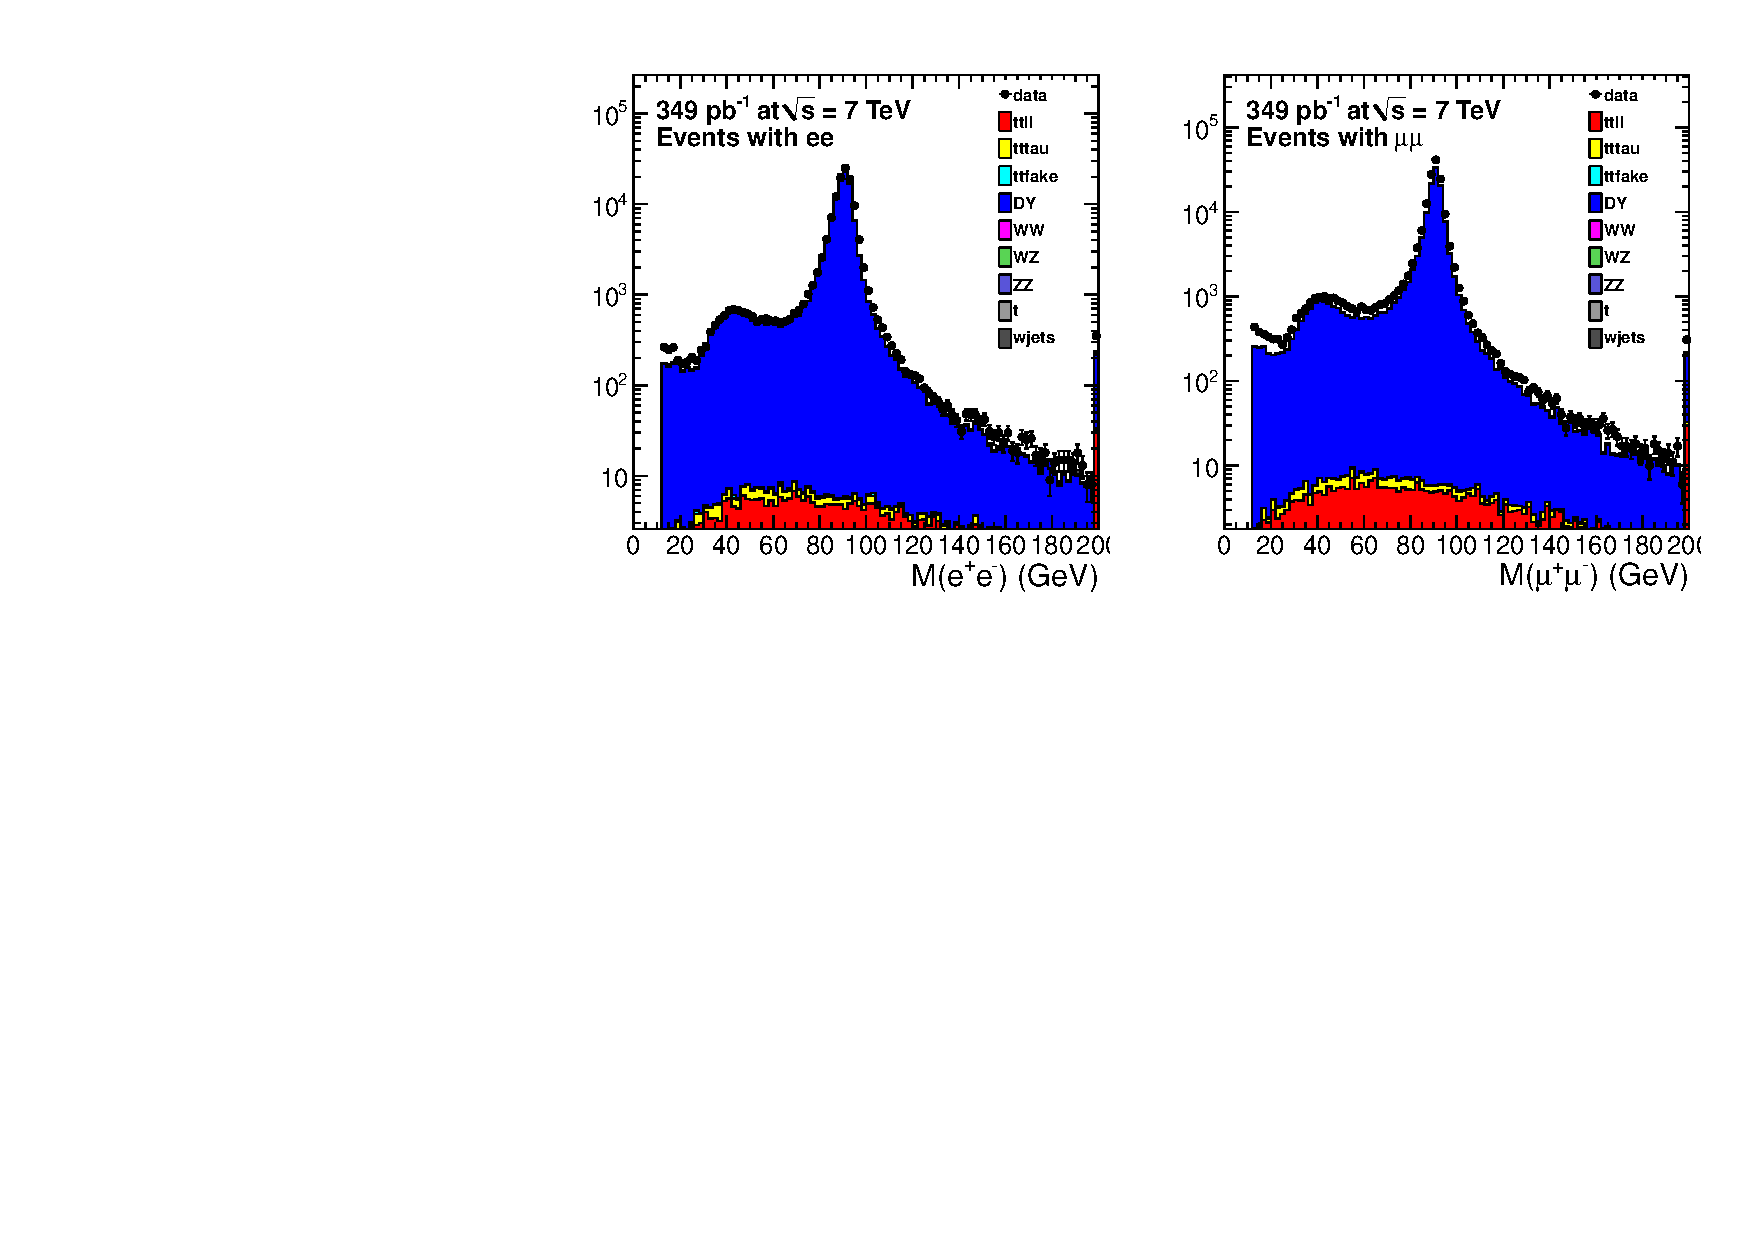
\includegraphics[width=1.0\linewidth]{plots/dilmass_349pb.pdf}
\caption{\label{fig:Z}\protect Distributions of dilepton mass in data and MC,
in the $ee$ channel (left) and $\mu\mu$ channel (right). 
}
\end{center}
\end{figure}


\begin{table}[htb]
\begin{center}
\caption{\label{tab:lepyields}
The data and MC yields in the $ee$ and $\mu\mu$ final states for events with 2 selected
leptons with invariant mass 76--106~GeV.
}
\begin{tabular}{l|cc}
\hline
         Sample   &           $ee$   &       $\mu\mu$   \\
\hline
data              &         110402   &         140191   \\
MC                &         107089   &         125998   \\
\hline
data/MC           &           1.03   &           1.11   \\
\hline
\end{tabular}
\end{center}
\end{table}

The data and MC dilepton mass distributions for events with 2 leptons passing the dilepton triggered 
\pt\ $>$ (20,10) GeV selection are displayed in Fig.~\ref{fig:Z}.
The yields of $Z$ events in the mass range 76--106~GeV are indicated in Table~\ref{tab:lepyields}. 
In data we observe a slight excess with respect to MC expectations, of 3\% (11\%) in the $ee$ ($\mu\mu$) channel,
which we attribute to uncertainties in trigger efficiency, lepton selection efficiency, and integrated
luminosity. We use the ratio of $Z \to \mu^+\mu^-$ to $Z \to e^+e^-$ yields in data to estimate the
ratio of muon to electron selection efficiencies, and find $R_{\mu e} = \rm{eff}(\mu)/\rm{eff}(e) = 1.13$.

